\documentclass[aspectratio=169,11pt]{beamer}

\usetheme{metropolis}
\usepackage{appendixnumberbeamer}
\usepackage{booktabs}
\usepackage{xspace}
\usepackage{listings}
\usepackage{tikz}
\usetikzlibrary{positioning, arrows.meta}
\usepackage{graphicx}
\graphicspath{{images/}}

\definecolor{avlnavy}{RGB}{35, 55, 85}
\definecolor{avlaccent}{RGB}{140, 100, 60}
\definecolor{avlgray}{RGB}{100, 105, 115}
\definecolor{avllight}{RGB}{248, 248, 250}

\setbeamercolor{progress bar}{fg=avlnavy}
\setbeamercolor{title separator}{fg=avlnavy}
\setbeamercolor{frametitle}{bg=avlnavy, fg=white}
\setbeamercolor{alerted text}{fg=avlaccent}
\setbeamercolor{block title}{bg=avlnavy!8, fg=avlnavy}
\setbeamercolor{block body}{bg=avllight}

\setbeamerfont{title}{size=\LARGE, series=\bfseries}
\setbeamerfont{subtitle}{size=\normalsize, series=\mdseries}
\setbeamerfont{frametitle}{size=\large, series=\bfseries}

\lstset{
  basicstyle=\ttfamily\footnotesize,
  keywordstyle=\color{avlnavy}\bfseries,
  commentstyle=\color{avlgray}\itshape,
  stringstyle=\color{avlaccent},
  backgroundcolor=\color{avllight},
  frame=single,
  framesep=4pt,
  rulecolor=\color{avlnavy!20},
  numbers=left,
  numberstyle=\tiny\color{avlgray},
  breaklines=true,
  showstringspaces=false,
  xleftmargin=2em,
  xrightmargin=1em,
}

\title{Using AI Tools in Mechatronics Projects}
\subtitle{A practical introduction}
\date{}
\author{Parsa Ghasemi}
\institute{Autonomous Vehicle Laboratory}

\begin{document}

\maketitle

% =========================================================
\begin{frame}{Overview}
  \begin{itemize}
    \setlength\itemsep{0.5em}
    \item What tools are available
    \item How to use them effectively
    \item Where they commonly make mistakes
    \item Live coding: building a motor controller
    \item Two demos combining AI with hardware
  \end{itemize}
\end{frame}

\begin{frame}{What This Talk Covers}
  This is a short practical guide. The goal is that you can open one of these tools tonight and use it for your own work.
  \vfill
  \begin{itemize}
    \setlength\itemsep{0.4em}
    \item We will not cover the underlying theory
    \item We will not compare every tool on the market
    \item We will focus on workflow and common pitfalls
  \end{itemize}
\end{frame}

% =========================================================
\section{Tools}
% =========================================================

\begin{frame}{Two Tools We Will Use}
  \begin{columns}[T,onlytextwidth]
    \begin{column}{0.48\textwidth}
      \begin{block}{Gemini CLI}
        \begin{itemize}
          \item Free
          \item 1{,}000 requests per day
          \item Google account sign-in
          \item Open source
        \end{itemize}
      \end{block}
    \end{column}
    \begin{column}{0.48\textwidth}
      \begin{block}{Claude Code}
        \begin{itemize}
          \item Paid (\$20/month)
          \item Generally stronger reasoning
          \item Good for embedded work
          \item Handles larger projects
        \end{itemize}
      \end{block}
    \end{column}
  \end{columns}
  \vfill
  Either tool works for everything shown today. The free option is a reasonable starting point.
\end{frame}

\begin{frame}{Gemini CLI}
  \begin{center}
    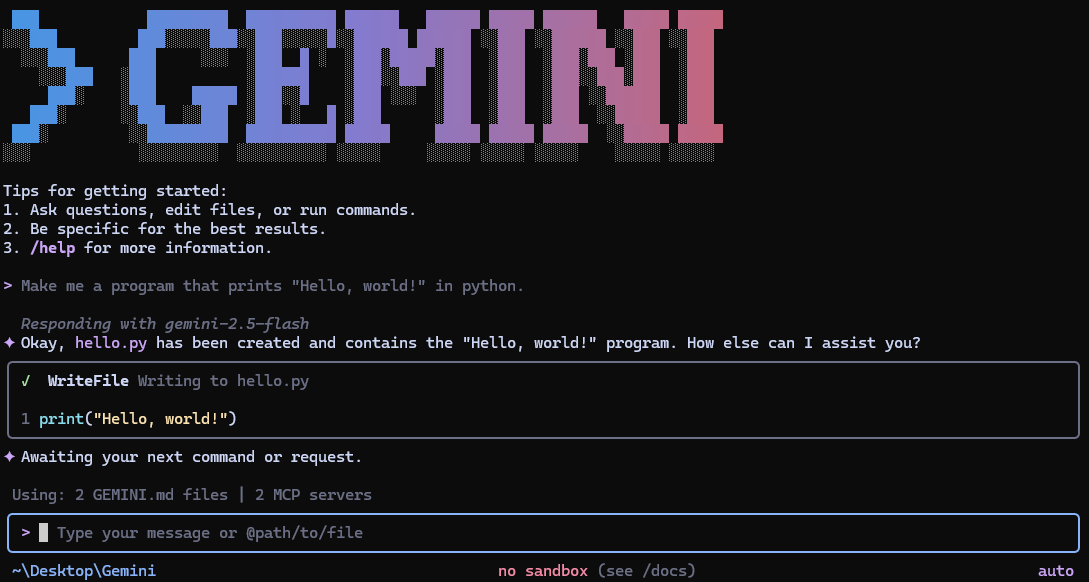
\includegraphics[width=0.72\textwidth]{gemini_cli.png}
  \end{center}
  \vfill
  \small A simple REPL in your terminal. You type what you want; it reads, writes, and edits files in your project.
\end{frame}

\begin{frame}{Claude Code}
  \begin{center}
    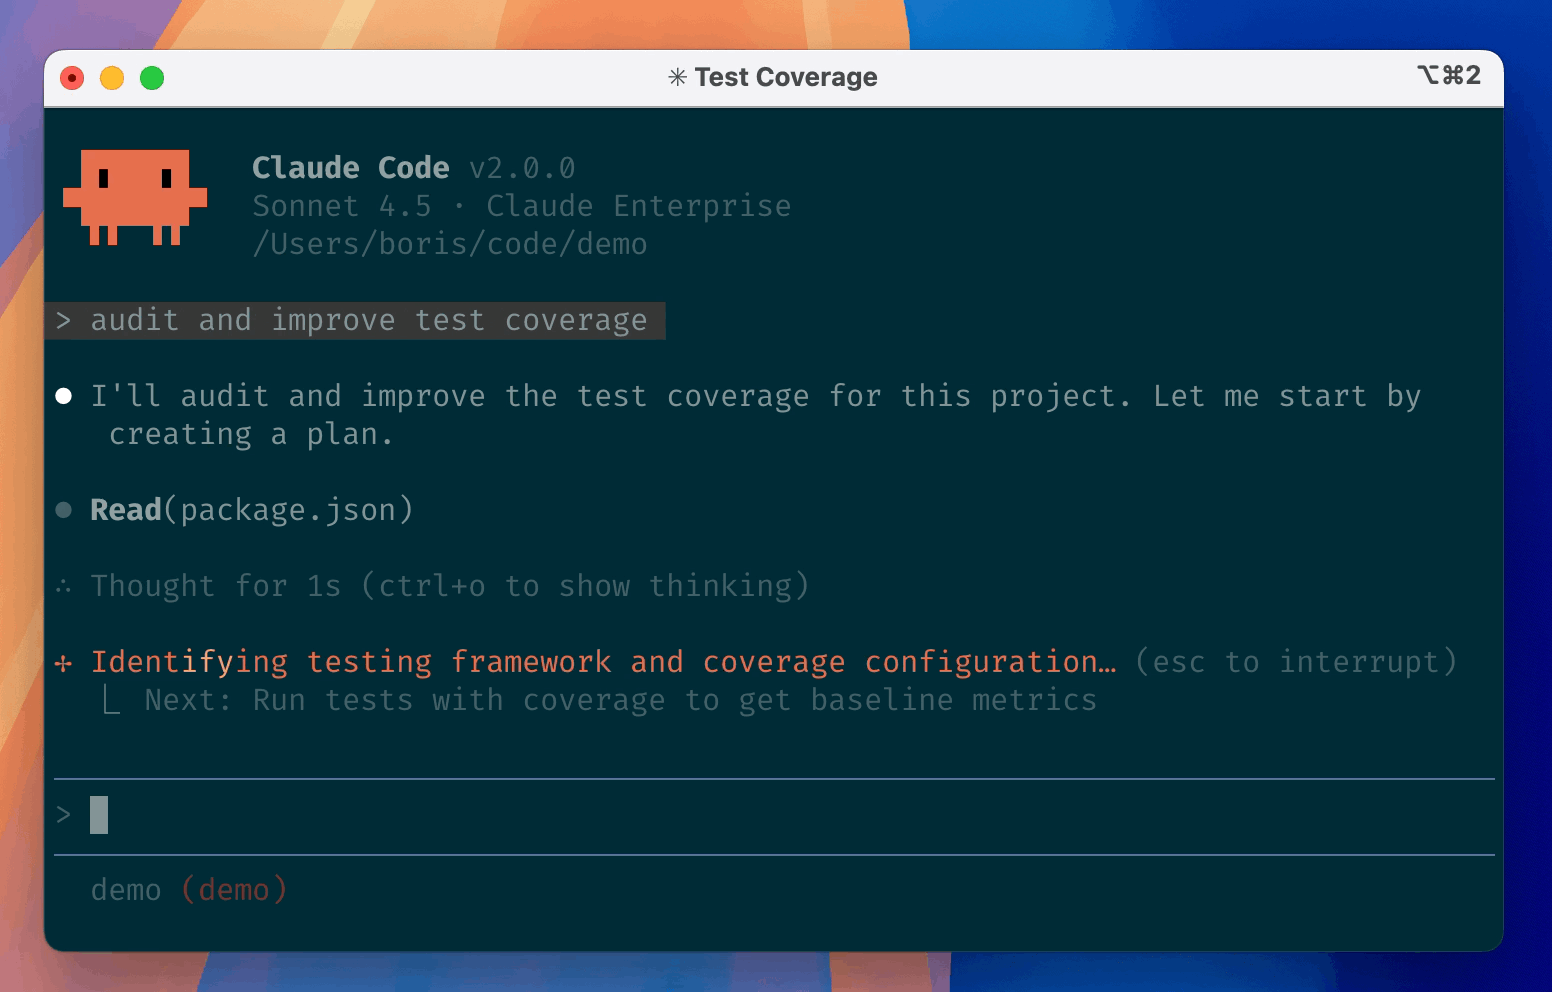
\includegraphics[width=0.55\textwidth]{claude_cli.png}
  \end{center}
  \vfill
  \small The same idea from Anthropic. Often better at longer tasks and embedded code, but requires a paid subscription.
\end{frame}

\begin{frame}{Why a Terminal Interface}
  Terminal-based AI tools differ from chat windows in a few practical ways:
  \vfill
  \begin{itemize}
    \setlength\itemsep{0.4em}
    \item They can read the files in your project directory
    \item They can edit files directly, without copy-paste
    \item They can run shell commands, including build and flash tools
    \item They keep context across a full working session
  \end{itemize}
\end{frame}

\begin{frame}{What an Agentic CLI Actually Does}
  \begin{center}
    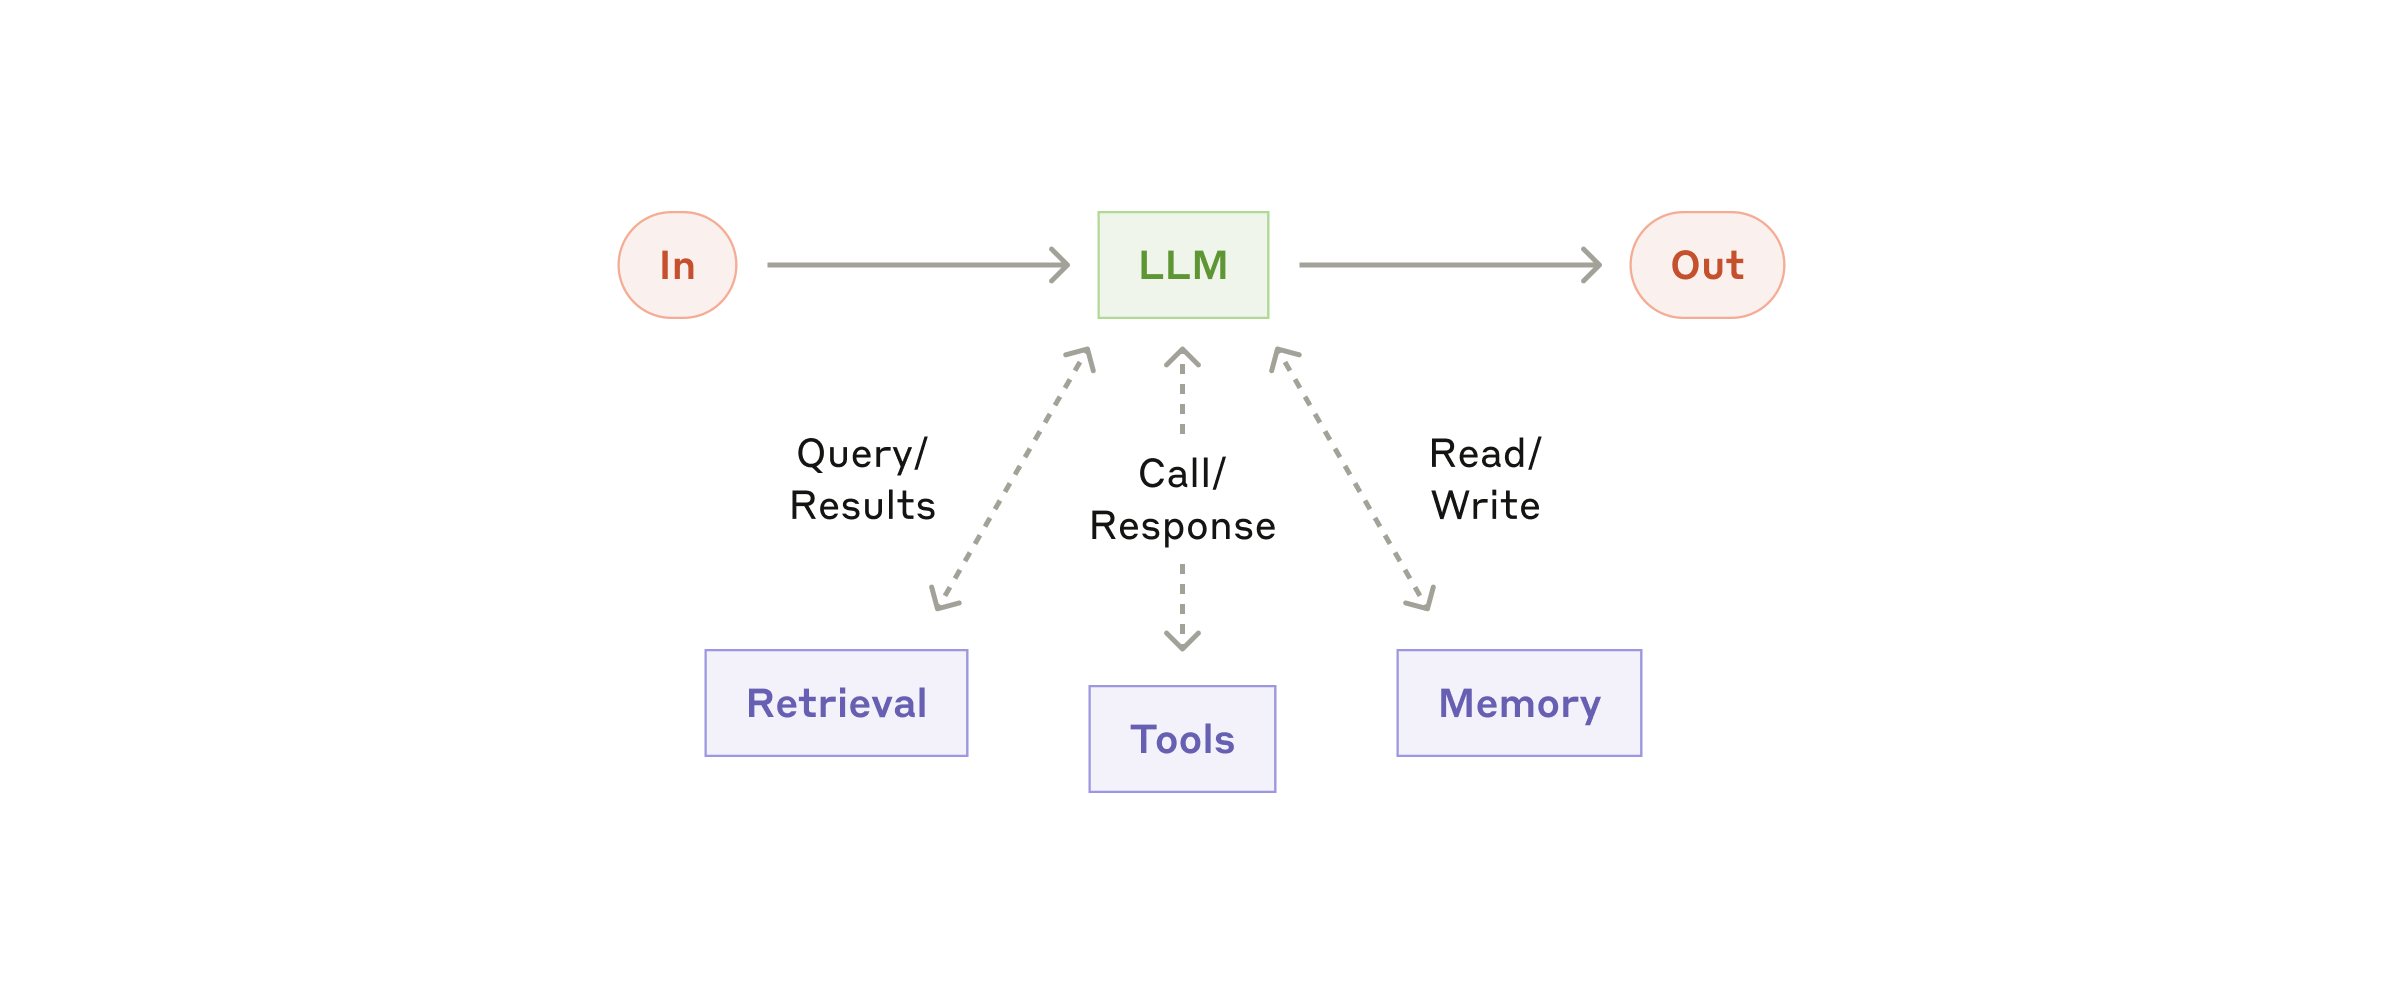
\includegraphics[width=0.78\textwidth]{augmented_llm.png}
  \end{center}
  \vfill
  \small The underlying language model is augmented with access to \textbf{tools} (shell, file edits, compilers), \textbf{retrieval} (your project files), and \textbf{memory} (session context). The CLI is the harness that wires these together.

  \hfill {\scriptsize \itshape Source: Anthropic, ``Building Effective Agents''}
\end{frame}

\begin{frame}{The Agentic Loop}
  \begin{center}
    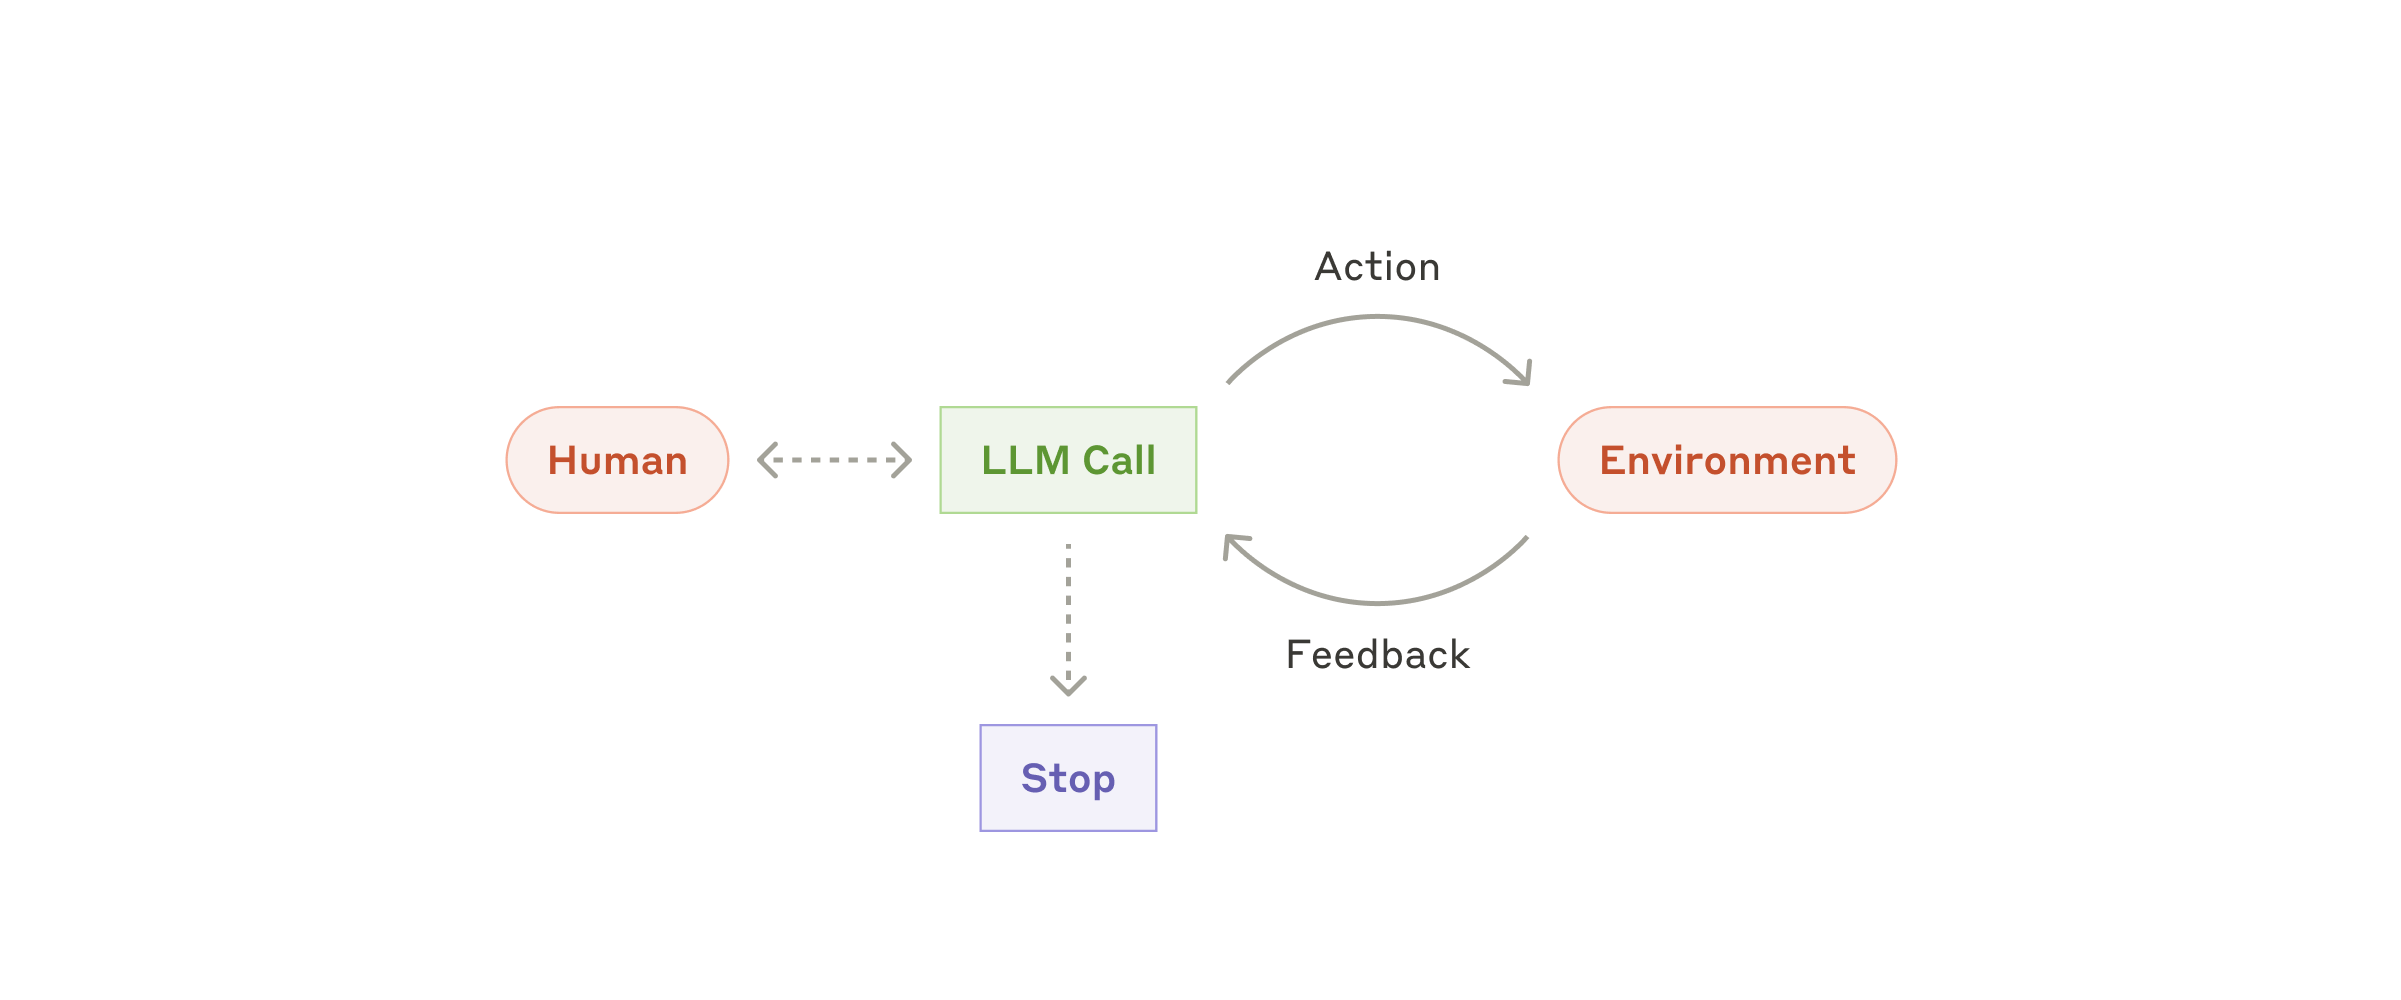
\includegraphics[width=0.78\textwidth]{autonomous_agent.png}
  \end{center}
  \vfill
  \small You state a goal; the model takes an action (edits a file, runs a command); it observes the feedback (error, output); and it iterates until the task is done or it asks you for help.

  \hfill {\scriptsize \itshape Source: Anthropic, ``Building Effective Agents''}
\end{frame}

\begin{frame}[fragile]{Installation (macOS / Linux)}
  \textbf{Prerequisite:} Node.js 18 or later, from \texttt{nodejs.org}
  \vspace{1em}
  \begin{lstlisting}
# Gemini CLI
npm install -g @google/gemini-cli
gemini

# Claude Code
npm install -g @anthropic-ai/claude-code
claude
  \end{lstlisting}
  \vfill
  On first run, sign in with a Google account (Gemini) or Claude account.
\end{frame}

\begin{frame}{Windows: Consider Using WSL}
  WSL (Windows Subsystem for Linux) provides a Linux environment inside Windows, without dual boot or a virtual machine.
  \vfill
  It is worth using because:
  \begin{itemize}
    \setlength\itemsep{0.4em}
    \item Most AI tooling is tested on Linux first
    \item Most tutorials online assume a Linux shell
    \item Path and permission issues are rarer
  \end{itemize}
  \vfill
  It is not required. Native Windows works too.
\end{frame}

\begin{frame}[fragile]{Installing WSL}
  \begin{enumerate}
    \setlength\itemsep{0.4em}
    \item Open PowerShell as Administrator
    \item Run:
      \begin{lstlisting}
wsl --install
      \end{lstlisting}
    \item Restart the computer
    \item On restart, Ubuntu opens. Set a username and password.
  \end{enumerate}
\end{frame}

\begin{frame}[fragile]{Installing the CLI Inside WSL}
  \begin{lstlisting}
curl -fsSL https://deb.nodesource.com/setup_20.x | sudo -E bash -
sudo apt install -y nodejs

sudo npm install -g @google/gemini-cli
gemini
  \end{lstlisting}
  \vfill
  The VS Code WSL extension is useful if you prefer a graphical editor while working inside Linux.
\end{frame}

% =========================================================
\section{Writing Effective Prompts}
% =========================================================

\begin{frame}{A Useful Prompt Structure}
  Prompts tend to work better when they include, in some form:
  \vfill
  \begin{enumerate}
    \setlength\itemsep{0.4em}
    \item A brief role or framing
    \item The specific context of your setup
    \item A clear task
    \item Relevant constraints
    \item Some form of verification
  \end{enumerate}
  \vfill
  These do not need to be labeled as such. The point is to give the tool enough information to answer precisely.
\end{frame}

\begin{frame}{An Example Prompt}
  \footnotesize
  \begin{quote}
    I am using a Teensy 4.1 with a DC motor driver on pins 3 and 4, and a quadrature encoder on pins 2 and 7.
    \medskip

    Please write an Arduino sketch that spins the motor one full rotation forward and then stops.
    \medskip

    Use the Encoder library. The encoder produces 5760 counts per revolution.
    \medskip

    Briefly explain each part of the code, and list the wiring.
  \end{quote}
\end{frame}

\begin{frame}{Vague Prompts vs Specific Prompts}
  \begin{columns}[T,onlytextwidth]
    \begin{column}{0.48\textwidth}
      \textbf{Vague}
      \vspace{0.4em}

      \itshape ``Write me motor code.''
      \vspace{0.8em}

      \normalfont
      Without context, the tool has to guess: which board, which driver, which pins, which libraries.
    \end{column}
    \begin{column}{0.48\textwidth}
      \textbf{Specific}
      \vspace{0.4em}

      \itshape ``I have a Teensy 4.1 with a motor driver on pins 3 and 4. Please write a sketch that spins forward for 2 seconds, stops, then reverses.''
      \vspace{0.8em}

      \normalfont
      Now the reply is targeted and usually runnable.
    \end{column}
  \end{columns}
\end{frame}

\begin{frame}{Providing Context}
  It is often helpful to share:
  \vfill
  \begin{itemize}
    \setlength\itemsep{0.4em}
    \item Relevant sections of a datasheet
    \item Your wiring, in a few lines of text
    \item A photo of the circuit
    \item The existing code you are editing
    \item The exact error message you encountered
  \end{itemize}
  \vfill
  A useful rule of thumb: if you would need to explain it to a classmate for them to help, the tool likely needs it too.
\end{frame}

% =========================================================
\section{Common Mistakes}
% =========================================================

\begin{frame}{Where These Tools Often Go Wrong}
  Even capable models make confident mistakes. Common ones include:
  \vfill
  \begin{itemize}
    \setlength\itemsep{0.4em}
    \item Incorrect pin numbers
    \item Unit errors (radians vs degrees, RPM vs rad/s)
    \item Function names that do not exist in the library
    \item Code written for a different board
    \item Part numbers that are not real
    \item Links that do not resolve
  \end{itemize}
\end{frame}

\begin{frame}[fragile]{A Small Example}
  Prompt: \itshape ``Write Arduino code to spin a motor at 50\% speed.''
  \vspace{0.5em}
  \begin{lstlisting}[language=C++]
int motorPin = 9;

void setup() {
  pinMode(motorPin, OUTPUT);
}

void loop() {
  analogWrite(motorPin, 50);  // 50% speed, right?
}
  \end{lstlisting}
\end{frame}

\begin{frame}{The Issue}
  \texttt{analogWrite} accepts values from \textbf{0 to 255}, not 0 to 100.
  \vfill
  A value of 50 corresponds to roughly 20\% duty cycle, not 50\%. The code compiles, the motor spins, and the behavior looks reasonable. It is simply not what was asked for.
\end{frame}

\begin{frame}{Ways to Catch These}
  A short checklist that helps:
  \vfill
  \begin{itemize}
    \setlength\itemsep{0.4em}
    \item Read each line before running it
    \item Compile early; syntax errors surface fake APIs quickly
    \item Test the simple cases (known input, known expected output)
    \item Confirm the wiring matches what the code expects
    \item Ask the tool to review its own code for bugs
  \end{itemize}
  \vfill
  Over time, you learn the kinds of mistakes a given tool tends to make.
\end{frame}

% =========================================================
\section{Live Coding}
% =========================================================

\begin{frame}{Why a Live Demo}
  Everything so far has been description. The purpose of coding live is:
  \vfill
  \begin{itemize}
    \setlength\itemsep{0.4em}
    \item To show the actual pace and rhythm of the workflow
    \item To show how mistakes appear and get corrected in practice
    \item To give you something to compare against when you try it yourself
    \item To connect what follows: both demos reuse this firmware
  \end{itemize}
\end{frame}

\begin{frame}{Building a Motor Controller}
  In the next few minutes, we will build a position-controlled motor from an empty folder, using only the terminal.
  \vfill
  \textbf{The plan:}
  \begin{enumerate}
    \setlength\itemsep{0.3em}
    \item Spin the motor
    \item Read the encoder
    \item Accept setpoints over serial
    \item Add a PID controller
  \end{enumerate}
\end{frame}

\begin{frame}{Hardware Setup}
  \begin{columns}[T,onlytextwidth]
    \begin{column}{0.55\textwidth}
      \begin{itemize}
        \setlength\itemsep{0.3em}
        \item Teensy 4.1, connected by USB
        \item Motor driver: RPWM on pin 3, LPWM on pin 4
        \item Encoder: channel A on pin 2, channel B on pin 7
        \item Gear motor, 5760 counts per revolution
        \item Bench power supply for the motor
      \end{itemize}
    \end{column}
    \begin{column}{0.42\textwidth}
      \centering
      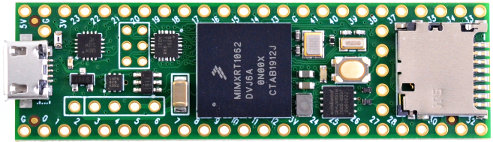
\includegraphics[width=\textwidth]{teensy.jpg}
      \vspace{0.3em}

      \scriptsize Teensy 4.1
    \end{column}
  \end{columns}
\end{frame}

\begin{frame}{Live Demo}
  \vfill
  \begin{center}
    \Large Live coding
    \vspace{0.8em}

    \normalsize\itshape A backup sketch is prepared in case of issues.
  \end{center}
  \vfill
\end{frame}

\begin{frame}{Brief Recap}
  \begin{itemize}
    \setlength\itemsep{0.4em}
    \item We started from an empty folder
    \item The CLI wrote the sketch, compiled it, and flashed the board
    \item A few mistakes appeared and were corrected with additional prompts
    \item The result is a working position controller
  \end{itemize}
  \vfill
  The workflow is the main point: describe, review, test, iterate.
\end{frame}

% =========================================================
\section{Two Further Demos}
% =========================================================

\begin{frame}{Demo 1 --- Vision to Motor}
  \begin{columns}[T,onlytextwidth]
    \begin{column}{0.55\textwidth}
      The webcam tracks a hand; the motor follows its position.
      \vspace{0.8em}

      \begin{itemize}
        \setlength\itemsep{0.3em}
        \item MediaPipe Hands (Google, free)
        \item A short Python script to read the webcam and send setpoints
        \item The same PID firmware on the Teensy
      \end{itemize}
      \vspace{0.8em}

      Approximate build time: a few hours.
    \end{column}
    \begin{column}{0.42\textwidth}
      \centering
      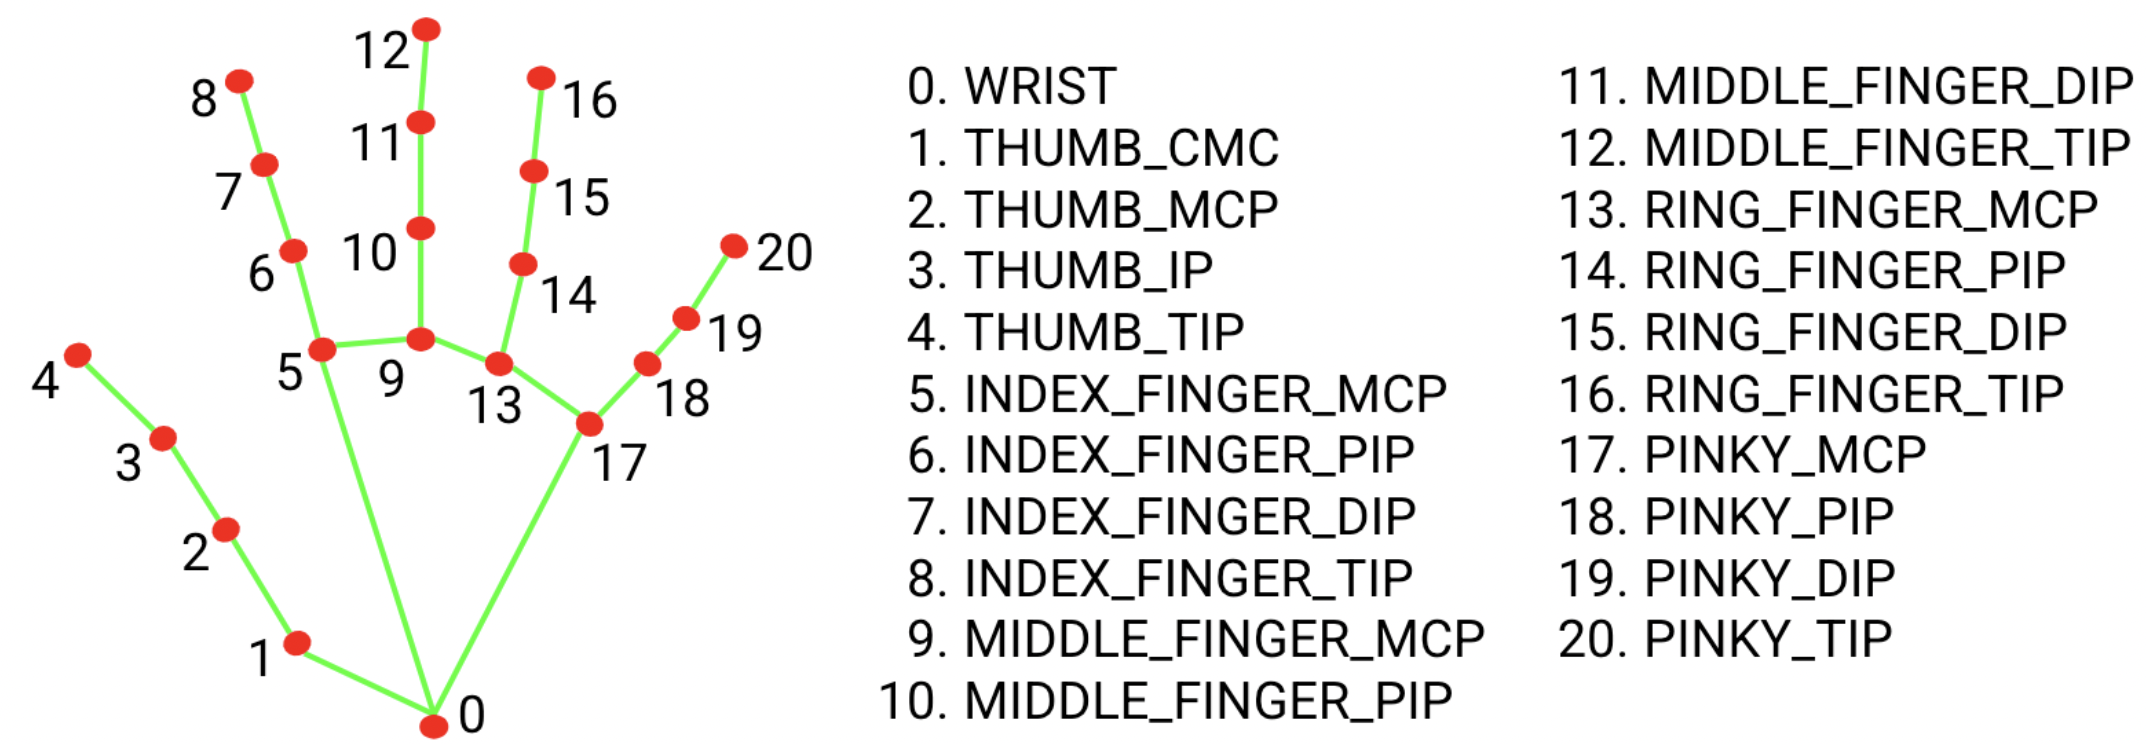
\includegraphics[width=\textwidth]{mediapipe.png}
      \vspace{0.3em}

      \scriptsize MediaPipe hand landmarks
    \end{column}
  \end{columns}
\end{frame}

\begin{frame}{Demo 1 --- Data Flow}
  \centering
  \vspace{0.5em}
  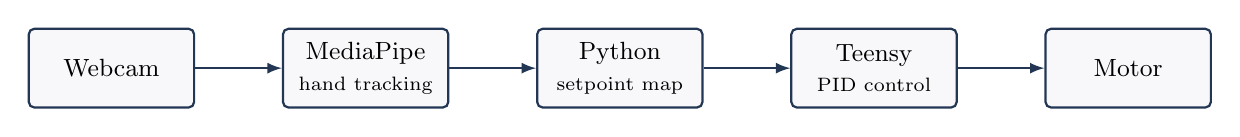
\begin{tikzpicture}[
    node distance=1.1cm,
    box/.style={rectangle, draw=avlnavy, thick, rounded corners=2pt,
                minimum width=2.1cm, minimum height=1cm, align=center,
                fill=avllight, font=\small},
    arrow/.style={->, thick, >=latex, color=avlnavy}
  ]
    \node[box] (cam)  {Webcam};
    \node[box, right=of cam]  (mp)  {MediaPipe\\\scriptsize hand tracking};
    \node[box, right=of mp]   (py)  {Python\\\scriptsize setpoint map};
    \node[box, right=of py]   (tn)  {Teensy\\\scriptsize PID control};
    \node[box, right=of tn]   (mot) {Motor};

    \draw[arrow] (cam) -- (mp);
    \draw[arrow] (mp)  -- (py);
    \draw[arrow] (py)  -- (tn);
    \draw[arrow] (tn)  -- (mot);
  \end{tikzpicture}
  \vfill
  \small Perception from the model; control from the microcontroller. Python and Teensy talk over USB serial.
\end{frame}

\begin{frame}{Demo 1: Live}
  \vfill
  \begin{center}
    \Large Vision to Motor
  \end{center}
  \vfill
\end{frame}

\begin{frame}{Demo 2 --- Voice to Motor}
  A spoken command is transcribed locally and mapped to a motor action.
  \vfill
  \begin{itemize}
    \setlength\itemsep{0.3em}
    \item OpenAI Whisper, running on the laptop (no internet needed)
    \item A short parser that recognizes a handful of commands
    \item The same Teensy firmware
  \end{itemize}
  \vfill
  Approximate build time: a couple of hours.
\end{frame}

\begin{frame}{Demo 2 --- Data Flow}
  \centering
  \vspace{0.5em}
  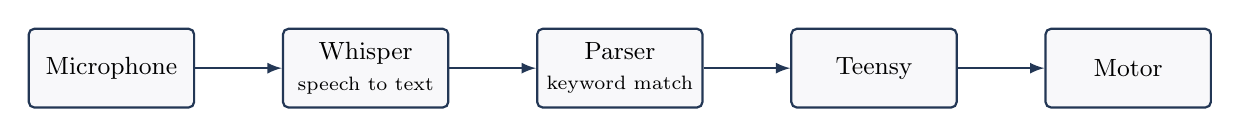
\begin{tikzpicture}[
    node distance=1.1cm,
    box/.style={rectangle, draw=avlnavy, thick, rounded corners=2pt,
                minimum width=2.1cm, minimum height=1cm, align=center,
                fill=avllight, font=\small},
    arrow/.style={->, thick, >=latex, color=avlnavy}
  ]
    \node[box] (mic) {Microphone};
    \node[box, right=of mic] (wh)  {Whisper\\\scriptsize speech to text};
    \node[box, right=of wh]  (pr)  {Parser\\\scriptsize keyword match};
    \node[box, right=of pr]  (tn)  {Teensy};
    \node[box, right=of tn]  (mot) {Motor};

    \draw[arrow] (mic) -- (wh);
    \draw[arrow] (wh)  -- (pr);
    \draw[arrow] (pr)  -- (tn);
    \draw[arrow] (tn)  -- (mot);
  \end{tikzpicture}
  \vfill
  \small Everything runs locally. No internet required after the first model download.
\end{frame}

\begin{frame}{Demo 2: Live}
  \vfill
  \begin{center}
    \Large Voice to Motor
    \vspace{0.8em}

    \normalsize\itshape A volunteer is welcome.
  \end{center}
  \vfill
\end{frame}

% =========================================================
\section{Suggestions}
% =========================================================

\begin{frame}{A Way to Get Started}
  \begin{enumerate}
    \setlength\itemsep{0.4em}
    \item Install Gemini CLI or Claude Code
    \item Ask it to walk you through a datasheet page
    \item Have it draft your next sketch, and read through carefully
    \item Paste a real bug and ask for a diagnosis
    \item Keep notes on the mistakes you notice
  \end{enumerate}
\end{frame}

\begin{frame}{A Few Things Worth Remembering}
  \begin{itemize}
    \setlength\itemsep{0.4em}
    \item These tools are useful; they are not a substitute for understanding
    \item Most of the productivity gain is on boilerplate and lookup
    \item Verification remains the engineer's responsibility
    \item Clear prompts generally matter more than picking the newest model
    \item The free options are sufficient to begin
  \end{itemize}
\end{frame}

% =========================================================

\begin{frame}{Thank You}
  \vfill
  \begin{center}
    Questions or discussion welcome.
    \vspace{1.5em}

    \small Parsa Ghasemi \\
    \small Autonomous Vehicle Laboratory \\
    \small github.com/Paarseus
  \end{center}
  \vfill
\end{frame}

\appendix

\begin{frame}[allowframebreaks]{References}
  \footnotesize
  \textbf{AI Tools}
  \begin{itemize}
    \item Gemini CLI \hfill \texttt{github.com/google-gemini/gemini-cli}
    \item Claude Code \hfill \texttt{claude.com/claude-code}
    \item Claude web chat \hfill \texttt{claude.ai}
    \item Cursor \hfill \texttt{cursor.com}
    \item GitHub Copilot (free for students) \hfill \texttt{education.github.com/pack}
  \end{itemize}
  \medskip
  \textbf{Demo Libraries}
  \begin{itemize}
    \item MediaPipe Hands \hfill \texttt{google.github.io/mediapipe}
    \item OpenAI Whisper \hfill \texttt{github.com/openai/whisper}
    \item Arduino CLI \hfill \texttt{arduino.github.io/arduino-cli}
    \item Encoder library \hfill \texttt{github.com/PaulStoffregen/Encoder}
    \item PID\_v1 library \hfill \texttt{github.com/br3ttb/Arduino-PID-Library}
  \end{itemize}
  \medskip
  \textbf{Embedded Toolchain}
  \begin{itemize}
    \item Teensyduino \hfill \texttt{pjrc.com/teensy/teensyduino.html}
    \item WSL \hfill \texttt{learn.microsoft.com/windows/wsl}
    \item usbipd-win \hfill \texttt{github.com/dorssel/usbipd-win}
  \end{itemize}
\end{frame}

\end{document}
